% Set the document class and theme
\documentclass{beamer}
\usetheme{CambridgeUS}
\setbeamertemplate{caption}[numbered]
\setbeamertemplate{theorems}[numbered]
\setbeamerfont{footnote}{size=\tiny}

\usepackage{./presentation_macros}

\addbibresource{references.bib}

% Add presentation data here

% Text in the square brackets `[]' are shown in the footer. If not mentioned,
% then text in the curly braces `{}' are used as theme defaults.

\title[Zone Encryption]{Zone Encryption with Anonymous Authentication for V2V
Communication \\
\small Jan Camenisch, Manu Drijvers, Anja Lehmann, Gregory Neven and Patrick
Towa}
\date{April 27, 2024}
\author{Gautam Singh}
\institute[IITH]{Indian Institute of Technology Hyderabad}

% Presentation begins here

\begin{document}
    \maketitle
    \tableofcontents
    \section{Introduction}
    
    \begin{frame}
        \frametitle{V2X Related Terminology}
        \begin{figure}
            \centering
            \resizebox{.8\textwidth}{!}{\begin{tikzpicture}[
    mindmap,
    concept color=red!55!black,
    text=white
]
    \node [concept] {\textbf{V2X}\\\small{Vehicle-to-Everything}}
    child[grow=150] {node[concept] {\textbf{V2D}\\\tiny{Vehicle-to-Device}}}
    child[grow=210] {node[concept] {\textbf{V2G}\\\tiny{Vehicle-to-Grid}}}
    child[grow=0] {
        node[concept] {\textbf{V2N}\\\tiny{Vehicle-to-Network}}
        child[grow=60] {node[concept] {\textbf{V2C}\\\tiny{Vehicle-to-Cloud}}}
        child[grow=120] {node[concept] {\textbf{V2P}\\\tiny{Vehicle-to-Pedestrian}}}
        child[concept color=green,grow=240,text=black] {node[concept] {\textbf{V2V}\\\tiny{Vehicle-to-Vehicle}}}
        child[concept color=green,grow=300,text=black] {node[concept] {\textbf{V2I}\\\tiny{Vehicle-to-Infrastructure}}}
    };
\end{tikzpicture}}
            \caption{A breakdown of V2X.}
        \end{figure}
    \end{frame}

    \begin{frame}
        \frametitle{Message Types in V2X}
        \begin{enumerate}
            \item<1-> \textbf{Cooperative Awareness Messages} (CAMs)
            \footcite{etsi-en-302-637} and \textbf{Basic Safety Messages} (BSMs)
            \footcite{J2735_202309V2XCommunications}.
            \begin{enumerate}
                \item Exchanged between vehicles to create awareness and support
                cooperative performance of vehicles in the road network.
                \item Includes status information such as time, position, speed,
                active systems, vehicle dimensions, etc.
            \end{enumerate}
            \item<2-> Other types of messages
            \begin{enumerate}
                \item \textbf{Signal Phase and Timing} (SPaT)
                \item \textbf{Roadside Infrastructure Information} (MAP)
            \end{enumerate} 
        \end{enumerate}
    \end{frame}

    \begin{frame}
        \frametitle{V2X and Cryptology}
        \begin{enumerate}
            \item<1-> CAMs broadcasted unencrypted in 5.9 GHz channel (ETSI ITS-G5).
            \begin{itemize}
                \item<2-> Frequently broadcast: 1 CAM per second in US, 10 per
                second in EU.
                \item<2-> Easy to intercept.
                \item<2-> Leak sensitive information about the vehicle owners.
                \item<3-> \textbf{Huge privacy concerns and threats!}
            \end{itemize}
            \item<4-> Encryption impractical, since CAMs \emph{must} be decrypted by
            nearby vehicles in a highly dynamic environment.
            \begin{itemize}
                \item But CAMs \emph{have to} be encrypted because of the data
                they carry!
            \end{itemize}
            \item<5-> Instead, focus on \emph{privacy-preserving authentication}.
            \begin{itemize}
                \item Ensuring a message is issued by a ``genuine'' vehicle.
                \item ``Genuine'' vehicles must be untraceable.
            \end{itemize}
        \end{enumerate}
    \end{frame}

    \begin{frame}
        \frametitle{V2X and Cryptology}
        \begin{enumerate}
            \item<1-> Deployed systems
            \begin{itemize}
                \item Use short-term \textbf{pseudonym certificates} (100 per
                week in EU, 20 per week in US), rotate between them.
                \item Trade-off between security (Sybil resistance), privacy and
                efficiency (storage and bandwidth costs).
            \end{itemize}
            \item<2-> Proposed systems
            \begin{itemize}
                \item Stronger privacy and security guarantees.
                \item Do not meet the \emph{stringent bandwidth constraint} of
                \textbf{300 bytes per CAM}, thus impractical.
            \end{itemize}
        \end{enumerate}
    \end{frame}

    \begin{frame}
        \frametitle{Motivation and Goals}
        \begin{enumerate}
            \item<1-> Unlimited privacy.
            \item<1-> Address problems of authenticity and confidentiality in
            combination \emph{for the first time}.
            \item<2-> Meet (bandwidth) requirements.
            \item<2-> Negligible storage and bandwidth overheads.
            \item<3-> Efficient encryption scheme (symmetric-key crypto).
            \item<3-> Better security guarantees (privacy, authenticity,
            confidentiality).
        \end{enumerate}
    \end{frame}

    \section{Preliminaries}

    \begin{frame}
        \frametitle{Preliminaries}
        \begin{enumerate}
            \item Pairing-based Cryptography
            \item Hardness Assumptions
            \begin{enumerate}
                \item Symmetric Discrete Logarithm (SDL) assumption
                \item Modified \(q\)-Strong Diffie-Hellman (q-MSDH-1) assumption
            \end{enumerate}
            \item Deterministic Authenticated Encryption (DAE)
            \item \red{PS Signatures}
            \item \red{Dynamic Group Signatures with Attributes (DGS+A)}
            \item<2-> \textbf{CS6190}
        \end{enumerate}
    \end{frame}

    \section{Zone Encryption}
    \begin{frame}
        \frametitle{Overall Flow of Zone Encryption}
        \begin{figure}[!ht]
            \centering
            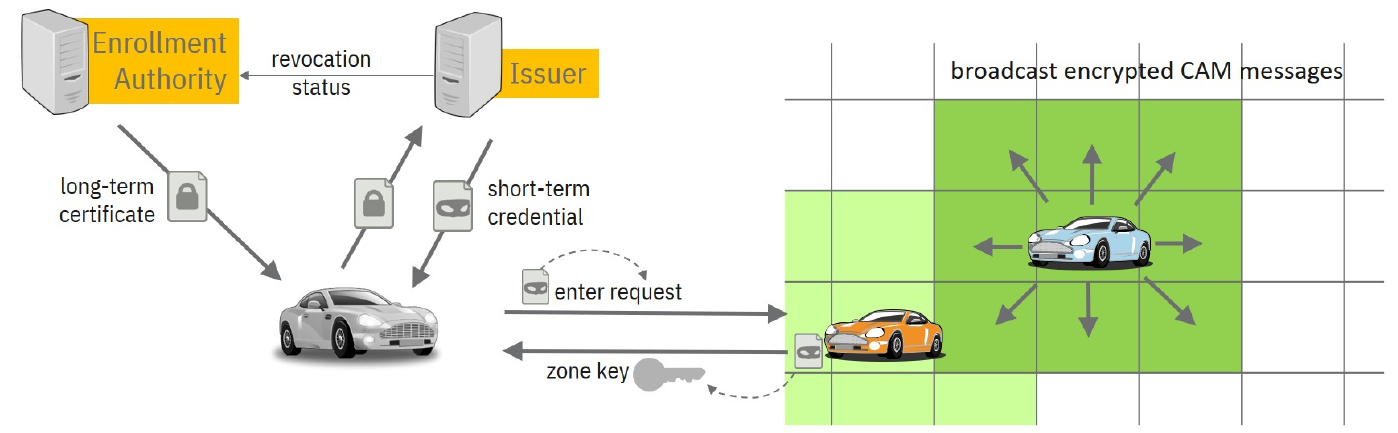
\includegraphics[width=\textwidth]{figs/ze_flow.png}
            \caption{Illustration of Zone Encryption with its Anonymous-Authentication Approach.}
        \end{figure}
    \end{frame}

    \begin{frame}
        \frametitle{Notation}
        \begin{table}[!ht]
            \centering
            \begin{tabular}{|c|c|}
                \hline
                \textbf{Notation} & \textbf{Meaning} \\
                \hline
                \(Z\) & Set of zones covering the road network \\
                \hline
                \(\cP\) & Payload/message space \\
                \hline
                \(Epoch\) & Set of epochs \\
                \hline
                \(T\) & Set of timestamps \\
                \hline
                \(K_{z,t}\) & Zone key for zone \(z\) at time \(t\) \\
                \hline
                \(L_K\) & List of zone keys known to a vehicle, stored as
                \(\brak{z,t,K_{z,t}}\) \\
                \hline
                \(\cE\) & Enrollment authority \\
                \hline
                \(\cI\) & Issuer \\
                \hline
                \(\cV \in \cbrak{0,1}^*\) & Vehicle identity \\
                \hline
                \(cert_{\cV}\) & Long-term certificate of \(\cV\) \\
                \hline
                \(cred_{\cV}\) & Short-term credential of \(\cV\) \\
                \hline
            \end{tabular}
        \end{table}
    \end{frame}

    \begin{frame}
        \frametitle{Zones, Epochs, Zone Keys}
        \begin{columns}
            \begin{column}{0.7\textwidth}
                \begin{enumerate}
                    \item A \emph{zone} \(z\) is a continuous geographical area
                    covering part of a road network (shown as squares alongside).
                    \item<2-> Each zone has a \emph{zone key} \(K_{z,t}\)
                    periodically refreshed after a time interval called an
                    \emph{epoch}.
                    \begin{itemize}
                        \item An epoch is denoted by \(\rbrak{\lsbrak{e,e+1}}\).
                        Each time instance \(t\) satisfies \(e \le t < e + 1\)
                        for a unique \(e\). This is denoted as \(e\brak{t}\).
                        \item Vehicles need \(K_{z,t}\) for secure communication
                        when they are in zone \(z\) at time \(t\).
                    \end{itemize}
                    \item<3-> Vechicles can communicate securely with other
                    vehicles in surrounding zones also.
                \end{enumerate}
            \end{column}
            \begin{column}<1->{0.3\textwidth}
                \begin{figure}
                    \centering
                    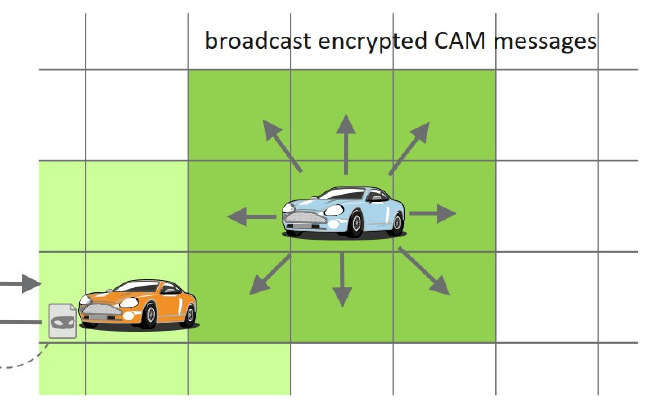
\includegraphics[width=\columnwidth]{figs/ze_zones.png}
                    \caption{A vehicle must have the zone keys of zones adjacent
                    to it. It can communicate with another vehicle if they share
                    a zone key.}
                \end{figure}
            \end{column}
        \end{columns}
    \end{frame}

    \begin{frame}
        \frametitle{Entities and Credentials}
        \begin{columns}
            \begin{column}{0.7\textwidth}
                \begin{enumerate}
                    \item An \emph{enrollment authority} \(\cE\) issues
                    \emph{long-term certificates} to vehicle \(\cV \in
                    \cbrak{0,1}^*\).
                    \begin{enumerate}
                        \item Long-term certificate \(cert_{\cV}\)
                        obtained.
                        \item Can be used to check revocation status.
                    \end{enumerate}
                    \item<2-> An \emph{issuer} \(\cI\) issues
                    \emph{short-term credentials} to vehicles every epoch.
                    \begin{enumerate}
                        \item Long-term credential \(cert_{\cV}\) used
                        here.
                        \item Short-term credential \(cred_{\cV}\)
                        obtained.
                        \item \(cred_{\cV}\) is valid only for the epoch
                        \(e\) in which it was issued.
                    \end{enumerate}
                \end{enumerate}
            \end{column}
            \begin{column}<1->{0.3\textwidth}
                \begin{figure}
                    \centering
                    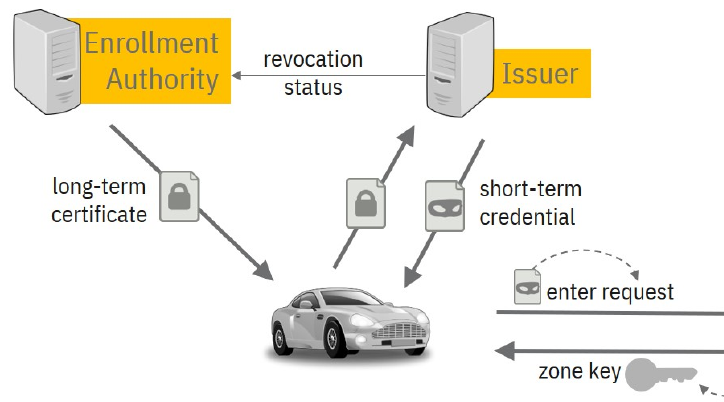
\includegraphics[width=\columnwidth]{figs/ze_entities.png}
                    \caption{Various entities and exchanged credentials in ZE.}
                \end{figure}
            \end{column}
        \end{columns}
    \end{frame}

    \begin{frame}
        \frametitle{Syntax of ZE}
        \begin{block}{Setup and Key Generation}
            \begin{enumerate}
                \item \(\mathsf{Setup}\brak{1^{\lambda},Z,Epoch,T} \rightarrow
                pp\)
                \item \(\mathsf{KG.E}\brak{pp} \rightarrow
                \brak{pk_{\cE},\brak{sk_{\cE},\red{st_{\cE}}}}\)
                \begin{itemize}
                    \item State keeps track of enrolled vehicles.
                \end{itemize}
                \item \(\mathsf{KG.I}\brak{pp} \rightarrow
                \brak{pk_{\cI},\brak{sk_{\cI},\red{st_{\cI}}}}\)
                \begin{itemize}
                    \item State keeps track of open messages sent during key
                    requests.
                \end{itemize}
            \end{enumerate}
        \end{block}
        \begin{block}<2->{Credential Issuance}
            \begin{enumerate}
                \item \(\abrak{\mathsf{Enroll.V}\brak{pk_{\cE},\cV}
                \leftrightharpoons
                \mathsf{Enroll.E}\brak{sk_{\cE},st_{\cE},\cV}} \rightarrow
                \abrak{cert_{\cV},st_{\cE}^{\prime}}\)
                \item
                \(\abrak{\mathsf{Authorize.V}\brak{\red{cert_{\cV}},e,pk_{\cI}}
                \leftrightharpoons
                \mathsf{Authorize.I}\brak{sk_{\cI},st_{\cI},\cV,e,\red{pk_{\cE}}}}
                \rightarrow \abrak{cred_{\cV},st_{\cI}^{\prime}}\)
                \begin{itemize}
                    \item<3-> Vehicle uses certificate to obtain credentials.
                    \item<3-> Issuer checks certificate using public key of
                    enrollment authority.
                \end{itemize}
            \end{enumerate}
        \end{block}
    \end{frame}

    \begin{frame}
        \frametitle{Syntax of ZE}
        \begin{block}{Entering and Exiting Zones}
            \begin{enumerate}
                \item \(\langle
                \mathsf{Enter.V}\brak{cred_{\cV},L_K,pk_{\cI},z,t,requester}
                \leftrightharpoons
                \mathsf{Enter.W}\brak{cred_{\cW_i},L_{K_i},pk_{\cI},z,t,responder_i}_{i\ge
                0} \rangle \rightarrow \abrak{L_K,\perp}\)
                \begin{itemize}
                    \item Why \(i \ge 0\)?
                \end{itemize}
                \item \(\mathsf{Exit}\brak{L_K,z,t} \rightarrow L_K^{\prime}\)
            \end{enumerate}
        \end{block}
        \begin{block}<2->{Sending and Receiving Payloads}
            \begin{enumerate}
                \item \(\mathsf{Send}\brak{L_K,P,\red{Y\subseteq Z},t}
                \rightarrow \gamma/\perp\)
                \item \(\mathsf{Receive}\brak{L_K,\gamma} \rightarrow P/\perp\)
                \item It's all symmteric key cryptography!
            \end{enumerate}
        \end{block}
    \end{frame}

    \begin{frame}
        \frametitle{Syntax of ZE}
        \begin{block}{Identity Escrow}
            \begin{enumerate}
                \item \(\mathsf{Open}\brak{sk_{\cI},st_{\cI},\red{m}}
                \rightarrow \cV/\perp\)
                \item \(m\) is a message that was sent during an execution of
                \textsf{Enter}.
                \item<2-> Only \(\cI\) can find which vehicle sent \(m\). Use
                cases
                \begin{itemize}
                    \item To revoke certificates of misbehaving vehicles.
                    \item To provide concrete court evidence.
                \end{itemize}
                \item<3-> Assuming identity escrow is rare, \textsf{Open} need
                not be efficient in terms of time/storage complexity.
            \end{enumerate}
        \end{block}
    \end{frame}

    \begin{frame}
        \frametitle{Security of ZE}
        \begin{enumerate}
            \item \textbf{Anonymity}: Ciphertexts and messages during
            \(\mathsf{Enter}\) do not reveal info about the vehicle that sent
            them.
            \begin{itemize}
                \item Not necessary for messages associated with
                \(\mathsf{Authorize}\). (Why?)
            \end{itemize}
            \item<2-> \textbf{Traceability}: If a vehicle knows \(K_{z,t}\), it
            must have entered zone \(z\) at time \(t\).
            \begin{itemize}
                \item Issuer can trace the messages during \(\mathsf{Enter}\) to
                long-term identity.
            \end{itemize}
            \item<3-> \textbf{Ciphertext Integrity}: An efficient adversary
            cannot compute a valid ciphertext \(\gamma\) for a given
            \(\brak{z,t}\) without knowing \(K_{z,t}\).
            \item<4-> \textbf{Payload-Hiding security against Chosen-Ciphertext
            Attacks (PH-CCA)}: No efficient adversary can infer about the
            underlying payload without knowing \(K_{z,t}\). 
        \end{enumerate}
    \end{frame}

    \begin{frame}
        \frametitle{Building Blocks of ZE}    
        \begin{enumerate}
            \item<1-> \(\mathsf{SIG}\): Signature scheme for long-term
            certificates.
            \item<2-> \(\mathsf{DGSA}\): Group signature scheme for short-term
            credentials.
            \item<3-> \(\mathsf{PKE}\): Public-key encryption for symmetric key
            exchange.
            \item<4-> \(\mathsf{SE}\): Symmetric-key encryption scheme for fast
            encryption of larger payloads.
            \item<5-> \(\mathsf{DAE}\): Deterministic Authenticated Encryption
            for wrapping symmetric payload keys with zone keys.
            \begin{itemize}
                \item Why not do DAE on payloads?
                \item<6-> \emph{Remember the CAM length constraint!}
            \end{itemize} 
        \end{enumerate}
    \end{frame}

    \begin{frame}
        \frametitle{Summary of ZE}
        \begin{table}[!ht]
            \begin{tblr}{
                width=\linewidth,
                colspec = {|X[c,m]|X[c,m]|X[c,m]|},
                hlines, vlines, measure=vbox,
            }
                \textbf{Parameter} & \textbf{Zone Encryption} & \textbf{C-ITS Proposal} \\
                Encrypted CAM & Yes & No \\
                Anonymity & Yes & No \\
                Pseudonyms per Week & Unlimited & 100 (EU) / 20 (US) \\
                CAM Authentication & DAE & ECDSA \\
                Overhead per CAM & 224 Bytes & 160 Bytes \\
                + per entered Zones & 284 (Request) / 300 (Response) Bytes & N/A
            \end{tblr}
            \caption{Comparison of zone encryption to current C-ITS proposals at
            a 128-bit security level.}
            \label{tab:ze-comp}
        \end{table}
    \end{frame}

    \section{Dynamic Group Signatures with Attributes}
    \begin{frame}
        \frametitle{Introduction to DGS+A}
        \begin{enumerate}
            \item<1-> \textbf{Group
            Signatures}\footcite{chaumGroupSignatures1991}: A scheme where a
            user can sign a message anonymously on behalf of the group.
            \begin{itemize}
                \item<2-> Group size and composition is fixed, thus impractical.
            \end{itemize}
            \item<3-> \textbf{Dynamic Group
            Signatures}\footcite{bonehShortGroupSignatures2004}: A scheme where
            users can additionally join and leave the group at any time.
            \item<4-> \textbf{Dynamic Group Signatures with Attributes}: Users
            obtain membership credentials corresponding to a set of their
            attributes by interacting with an issuer. Signatures are verified
            w.r.t. attributes.
            \begin{itemize}
                \item<5-> Other attributes of the user need not be revealed.
            \end{itemize}
            \item<6-> DGS+A using
            \(\mathsf{PS}\)\footcite{pointchevalShortRandomizableSignatures2015}
            scheme.
            \begin{itemize}
                \item Can sign \(k\) message blocks \red{at once}.
                \item No hash functions needed and signatures are
                \red{randomizable}.
                \item Also doubles up as a \red{ZKPoK} of \(\sigma\) on \(m\).
            \end{itemize}
        \end{enumerate}
    \end{frame}

    \begin{frame}
        \frametitle{Syntax of DGS+A}
        \textbf{Note}: An \emph{issuer} \(\cI\) is a trusted party that issues
        credentials to users and can find the user that generated a given
        signature for a given message.
        \begin{block}{Setup and Key Generation}
            \begin{enumerate}
                \item \(\mathsf{Setup}\brak{1^{\lambda}, k} \rightarrow pp\):
                Generate public parameters.
                \item \(\mathsf{KG.I}\brak{pp} \rightarrow
                \brak{pk,\brak{sk,st}}\): Generate key pair for \(\cI\).
            \end{enumerate}
        \end{block}
        \begin{block}{Credential Issuance}
            \(\abrak{\mathsf{Issue.I}\brak{sk, st, id, A = \brak{a_i}_{i=1}^k} \leftrightharpoons \mathsf{Issue.U}\brak{id, A, pk}}
            \rightarrow cred\): Interactive protocol between a user \(\cU\) 
            and issuer \(\cI\) to obtain credentials \(cred\).
        \end{block}
    \end{frame}

    \begin{frame}{Syntax of DGS+A}
        \begin{block}{Signing and Verification}
            \begin{enumerate}
                \item \(\mathsf{Auth}\brak{pk, cred, m} \rightarrow tok\):
                Generate an \emph{authentication token} or signature on \(m\).
                \item \(\mathsf{Vf}\brak{pk, m, A, tok} \rightarrow b \in
                \cbrak{0,1}\): Verify whether \(tok\) has been properly
                generated for the given \(m\) and \(A\).
            \end{enumerate}
        \end{block}
        \begin{block}{Opening}
            \(\mathsf{Open}\brak{sk, st, m, A, tok} \rightarrow id/\perp\):
            Check whether \(tok\) was generated properly and recover the
            identity \(id\) of the user that generated \(tok\).
            
            \textbf{Note}: Time complexity of \(\mathsf{Open}\) is
            \(\cO\brak{\abs{ID}}\).
        \end{block}
        \begin{enumerate}
            \item \textbf{Security Properties}: Correctness, Traceability,
            Anonymity.
            \item \textbf{Application to ZE}: 216 Byte token size at 128-bit
            security level.
            \item Extension to threshold opening.
        \end{enumerate}
    \end{frame}

    \section{Conclusion}
    \begin{frame}
        \frametitle{Challenges and Future Improvements}
        \begin{enumerate}
            \item<1-> \textbf{Key Agreement Strategy}
            \begin{itemize}
                \item Which vehicle should reply to an entering vehicle?
                \item How to handle key clusters due to transmission loss?
                \item How to refresh zone keys (and who will generate them)?
            \end{itemize}
            \item<2-> \textbf{Robustness / Implementation Details}
            \begin{itemize}
                \item Encrypting payloads under zone keys in a region.
                \item Overlapping time periods for smooth transition.
                \item Robust communication medium and retransmission mechanisms.
            \end{itemize}
            \item<3-> Do we \emph{really} need to encrypt CAMs?
            \begin{itemize}
                \item Google (Maps) may already be profiling us!
                \item Focus on more sensitive messages and information sent less
                frequently.
                \item Avoid complexities in implementation of ZE.
            \end{itemize}
        \end{enumerate}
    \end{frame}

    \section{Summary}
    \begin{frame}
        \frametitle{Summary}
        \begin{enumerate}
            \item<1-> Brief Introduction on V2X.
            \begin{itemize}
                \item Services of V2X
                \item Standards involved in V2X
                \item V2X and cryptography. \emph{Huge discrepancies}
            \end{itemize}
            \item<2-> Zone Encryption
            \begin{itemize}
                \item Motivation and goals
                \item Overall flow
                \item Syntax
                \item Building blocks
                \item Security properties
                \item Comparison to other proposals
            \end{itemize}
            \item<3-> DGS+A
            \begin{itemize}
                \item Syntax
                \item Instantiation from PS
                \item Application to ZE
            \end{itemize}
        \end{enumerate}
    \end{frame}

    \appendix
    \section{Pointcheval-Sanders Signatures}
    \begin{frame}
        \frametitle{Pointcheval-Sanders Signatures}
        Consider \(\Gamma = \brak{q, \bG_0, \bG_1, \bG_T, e: \bG_0 \times \bG_1
        \rightarrow \bG_T} \leftarrow \mathsf{G}\brak{1^{\lambda}}\), where
        \(\mathsf{G}\) is a type-3 pairing group generator and \(\lambda\) is
        the \emph{security parameter}, \(\mathsf{PS}\) consists of the following
        algorithms.
        \begin{algorithm}[H]
            \caption{\(\mathsf{PS.KG}\)}
            \label{alg:ps-kg}
            \begin{algorithmic}[1]
                \Require{Pairing group \(\Gamma\) and number of message blocks \(k\).}
                \Ensure{Signing and verification key \(\brak{vk,sk}\).}
                \State Generate \(g_1 \in_R \bG_1\), \(x, y_1, \ldots, y_{k+1} \in_R \bZ_q\).
                \State Compute \(X \gets g_1^x\) and \(Y_j \gets g_1^j\) for \(j \in \cbrak{1, \ldots, k+1}\).
                \State \Return \(sk \gets \brak{x, y_1, \ldots, y_{k+1}}\) and \(vk \gets \brak{X, Y_1, \ldots, Y_{k+1}}\).
            \end{algorithmic}
        \end{algorithm}
    \end{frame}

    \begin{frame}
        \frametitle{Pointcheval-Sanders Signatures}
        \begin{algorithm}[H]
            \caption{\(\mathsf{PS.Sign}\)}
            \label{alg:ps-sign}
            \begin{algorithmic}[1]
                \Require{Signing key \(sk\) and message \(m = \brak{m_1, \ldots, m_k}\).}
                \Ensure{Signature \(\sigma\) on \(m\).}
                \State Generate \(h \in_R \bG_1, m^{\prime} \in_R \bZ_q\).
                \State \Return \(\sigma \gets \brak{m^{\prime}, h, h^{x + \sum_{j=1}^ky_jm_j + y_{k+1}m^{\prime}}}\).
            \end{algorithmic}
        \end{algorithm}

        \begin{algorithm}[H]
            \caption{\(\mathsf{PS.Vf}\)}
            \label{alg:ps-vf}
            \begin{algorithmic}[1]
                \Require{Verification key \(vk\), message \(m = \brak{m_1, \ldots, m_k}\), signature \(\sigma = \brak{m^{\prime}, \sigma_1, \sigma_2}\) on \(m\).}
                \Ensure{\(b \in \cbrak{0, 1}\).}
                \State \Return \(b \gets e\brak{\sigma_1, X\prod_{j=1}^kY_j^{m_j}Y_{k+1}^{m^{\prime}}} \stackrel{?}{=} e\brak{\sigma_2, g_1}\)
            \end{algorithmic}
        \end{algorithm}
    \end{frame}
\end{document}
